\documentclass[11pt, aspectratio=169]{beamer}
\usetheme{Madrid}

\usepackage[utf8]{inputenc}
\usepackage[italian]{babel}
\usepackage{amsmath, amssymb}
\usepackage{graphicx}
\usepackage{booktabs}

% Comandi personalizzati
\newcommand{\uno}{\mathbf{1}}
\newcommand{\Prob}{\mathbb{P}}
\newcommand{\N}{\mathbb{N}}

\title{Modello SIR come Catena di Markov a Tempo Discreto}
\subtitle{Modelli Probabilistici}
\author{Francesco Castaldi}
\institute{Università di Bologna}
\date{A.A. 2025/2026}

\begin{document}

% SLIDE 1
\begin{frame}
    \titlepage
\end{frame}

% SLIDE 2
\begin{frame}{Introduzione}
    \begin{itemize}
        \item Il modello SIR descrive la diffusione di un'infezione in una popolazione chiusa.
        \item L'evoluzione futura dipende \textbf{solo dallo stato presente} $\rightarrow$ proprietà di Markov.
        \item Lo spazio degli stati è \textbf{finito} $\rightarrow$ catena di Markov a tempo discreto.
        \item Il problema non è epidemiologico: è un pretesto per applicare il formalismo matematico.
    \end{itemize}
    \vspace{0.5cm}
    \textbf{Riferimento}: Capitolo 7 del corso — Catene di Markov a tempo discreto.
\end{frame}

% SLIDE 3
\begin{frame}{Obiettivo}
    \begin{enumerate}
        \item \textbf{Costruire} la catena di Markov SIR: spazio degli stati, probabilità di transizione, matrice $P$.
        \item \textbf{Classificare} gli stati: identificare assorbenti e transitori.
        \item \textbf{Simulare} l'evoluzione con Monte Carlo per stimare:
        \begin{itemize}
            \item tempo medio di estinzione $\tau$;
            \item picco medio degli infetti;
            \item numero finale di rimossi $R_\infty$.
        \end{itemize}
    \end{enumerate}
\end{frame}

% SLIDE 4
\begin{frame}{Catene di Markov (Cap. 7)}
    \textbf{Definizione}: Processo stocastico $\{X_t\}$ a tempo discreto con la \textbf{proprietà di Markov}:
    \[ \Prob(X_{t+1} \mid X_t, X_{t-1}, \dots, X_0) = \Prob(X_{t+1} \mid X_t) \]
    
    \textbf{Matrice di transizione P}: $P(i,j) =$ probabilità di andare da $i$ a $j$ in un passo.
    \begin{itemize}
        \item $P$ è \textbf{stocastica}: $\sum_j P(i,j) = 1$ per ogni $i$.
    \end{itemize}
    
    \textbf{Stato assorbente}: $P(i,i) = 1$. Una volta entrato, non si esce più.
\end{frame}

% SLIDE 5
\begin{frame}{Modello SIR}
    Popolazione chiusa di \textbf{N individui}. Tre compartimenti:
    
    \vspace{0.3cm}
    \begin{center}
    \begin{tabular}{lll}
        \toprule
        Simbolo & Nome & Descrizione \\
        \midrule
        $S_t$ & Suscettibili & Possono essere infettati \\
        $I_t$ & Infetti & Possono trasmettere l'infezione \\
        $R_t$ & Rimossi & Guariti, immuni, non infettivi \\
        \bottomrule
    \end{tabular}
    \end{center}
    \vspace{0.3cm}
    
    \textbf{Vincolo}: $S_t + I_t + R_t = N$ per ogni $t$.
    
    \textbf{Stato}: $X_t = (S_t, I_t, R_t)$.
\end{frame}

% SLIDE 6
\begin{frame}{Spazio degli stati}
    \textbf{Definizione}: $E = \{(s, i, r) \in \N_0^3 : s + i + r = N\}$
    
    \textbf{Cardinalità}: $|E| = \binom{N+2}{2} = \frac{(N+1)(N+2)}{2}$
    
    \textbf{Esempi}:
    \begin{itemize}
        \item $N = 3 \Rightarrow |E| = 10$ stati
        \item $N = 100 \Rightarrow |E| = 5151$ stati
    \end{itemize}
    
    Lo spazio è \textbf{finito} $\rightarrow$ siamo nel caso classico delle catene a spazio finito (Cap. 7).
    
    \vspace{0.2cm}
    Per $N$ piccolo la matrice $P$ si calcola esplicitamente. Per $N$ grande si usa la simulazione Monte Carlo.
\end{frame}

% SLIDE 7
\begin{frame}{Probabilità di transizione}
    \textbf{Contagio}: $C_t \sim \text{Binomiale}\left(S_t, \beta \frac{I_t}{N}\right)$
    
    \textbf{Guarigione}: $G_t \sim \text{Binomiale}(I_t, \gamma)$
    
    \textbf{Aggiornamento}:
    \begin{align*}
        S_{t+1} &= S_t - C_t \\
        I_{t+1} &= I_t + C_t - G_t \\
        R_{t+1} &= R_t + G_t
    \end{align*}
    
    \textbf{Parametri}:
    \begin{itemize}
        \item $\beta \in [0,1]$ : tasso di trasmissione
        \item $\gamma \in [0,1]$ : tasso di guarigione
    \end{itemize}
    
    Contagio e guarigione sono \textbf{indipendenti}. La probabilità di transizione è il prodotto delle due Binomiali.
\end{frame}

% SLIDE 8
\begin{frame}{Esempio: N=3, $\beta=0.5, \gamma=0.3$}
    Stato iniziale: \textbf{(2, 1, 0)}
    
    \vspace{0.3cm}
    \begin{center}
    \begin{tabular}{ccll}
        \toprule
        $C$ (contagi) & $G$ (guarigioni) & Stato finale & Probabilità \\
        \midrule
        0 & 0 & (2, 1, 0) & 0.486 \\
        0 & 1 & (2, 0, 1) & 0.208 \\
        1 & 0 & (1, 2, 0) & 0.194 \\
        1 & 1 & (1, 1, 1) & 0.083 \\
        \bottomrule
    \end{tabular}
    \end{center}
    \vspace{0.3cm}
    
    $\sum \text{probabilità} = 1$ \checkmark \textemdash \ riga stocastica.
\end{frame}

% SLIDE 9
\begin{frame}{Matrice di transizione P}
    \textbf{Elemento generico}:
    \begin{equation*}
    P((s,i,r), (s',i',r')) = \sum_c \sum_g \text{Bin}\left(s; c, \frac{\beta i}{N}\right) \cdot \text{Bin}(i; g, \gamma) \cdot \uno_{A}
    \end{equation*}
    dove $A = \{s' = s-c, i' = i+c-g, r' = r+g\}$.
    
    \textbf{Proprietà}:
    \begin{itemize}
        \item $P$ è \textbf{stocastica}: le righe sommano a 1.
        \item Per $N=3$: $P$ è $10 \times 10$, calcolabile esplicitamente.
        \item Per $N=100$: $5151$ stati $\rightarrow \sim 26\text{M}$ elementi $\rightarrow$ si procede per simulazione.
    \end{itemize}
    
    \textit{La matrice esiste sempre matematicamente, anche quando non la scriviamo per intero in memoria.}
\end{frame}

% SLIDE 10
\begin{frame}{Classificazione degli stati}
    \textbf{Stato $(s, i, r)$ con $i = 0 \rightarrow$ assorbente}
    \begin{itemize}
        \item $P((s,0,r), (s,0,r)) = 1$
        \item Non ci sono infetti: nessun contagio, nessuna guarigione.
    \end{itemize}
    
    \textbf{Stato $(s, i, r)$ con $i > 0 \rightarrow$ transitorio}
    \begin{itemize}
        \item Da ogni stato con $I>0$ si raggiunge un assorbente.
        \item Non si può tornare a $I>0$ dopo l'assorbimento.
    \end{itemize}
    
    \textbf{Conseguenza}: l'estinzione dell'infezione è \textbf{certa}: $\Prob(\tau < \infty) = 1$. \\
    \textit{La catena è una catena assorbente (Cap. 7).}
\end{frame}

% SLIDE 11
\begin{frame}{Algoritmo di simulazione (Monte Carlo)}
    \begin{enumerate}
        \item Inizializza: $S_0 = N - I_0, I_0 = I_0, R_0 = 0$
        \item \textbf{Loop} per $t = 0, 1, \dots, T_{max}$:
        \begin{enumerate}
            \item Se $I_t = 0 \rightarrow$ fermati (estinzione)
            \item $C_t \sim \text{Binomiale}(S_t, \beta \cdot I_t / N)$
            \item $G_t \sim \text{Binomiale}(I_t, \gamma)$
            \item $S_{t+1} = S_t - C_t$
            \item $I_{t+1} = I_t + C_t - G_t$
            \item $R_{t+1} = R_t + G_t$
        \end{enumerate}
        \item Restituisci traiettoria $(S_t, I_t, R_t)$
    \end{enumerate}
    
    \textbf{Parametri}: $N=100, \beta=0.2, \gamma=0.1, I_0=5, T_{max}=200, M=1000$ \\
    \textbf{Numero Riproduttivo}: $R_0 = \beta/\gamma = 2.0$ (ogni infetto genera 2 nuovi infetti in media).
\end{frame}

% SLIDE 12
\begin{frame}[fragile]{Codice Python — Passo della catena}
\begin{verbatim}
import numpy as np

N, BETA, GAMMA, I0 = 100, 0.2, 0.1, 5
T_MAX, M = 200, 1000

def next_state(s, i, r, n=N, beta=BETA, gamma=GAMMA):
    if i == 0:
        return s, 0, r
    p_si = beta * i / n
    new_infections = np.random.binomial(s, p_si)
    recoveries = np.random.binomial(i, gamma)
    
    return (s - new_infections, 
            i + new_infections - recoveries, 
            r + recoveries)
\end{verbatim}
\end{frame}

% SLIDE 13
\begin{frame}{Risultati numerici ($M=1000$)}
    \begin{center}
    \begin{tabular}{lcccc}
        \toprule
        Indicatore & Media & Dev.std & Min & Max \\
        \midrule
        Picco $I_{max}$ & 29.4 & 8.7 & 6 & 52 \\
        $\tau$ (tempo estinzione) & 68.3 & 18.2 & 12 & 124 \\
        $R_\infty$ (rimossi finali) & 87.2 & 9.5 & 34 & 100 \\
        \bottomrule
    \end{tabular}
    \end{center}
    
    \textbf{Osservazioni}:
    \begin{itemize}
        \item Forte variabilità tra simulazioni (natura stocastica del processo markoviano).
        \item In media l'87\% della popolazione viene infettata.
        \item Il tempo di estinzione varia da 12 a 124 passi.
    \end{itemize}
\end{frame}

% SLIDE 14
\begin{frame}{Singola traiettoria SIR}
    \begin{center}
        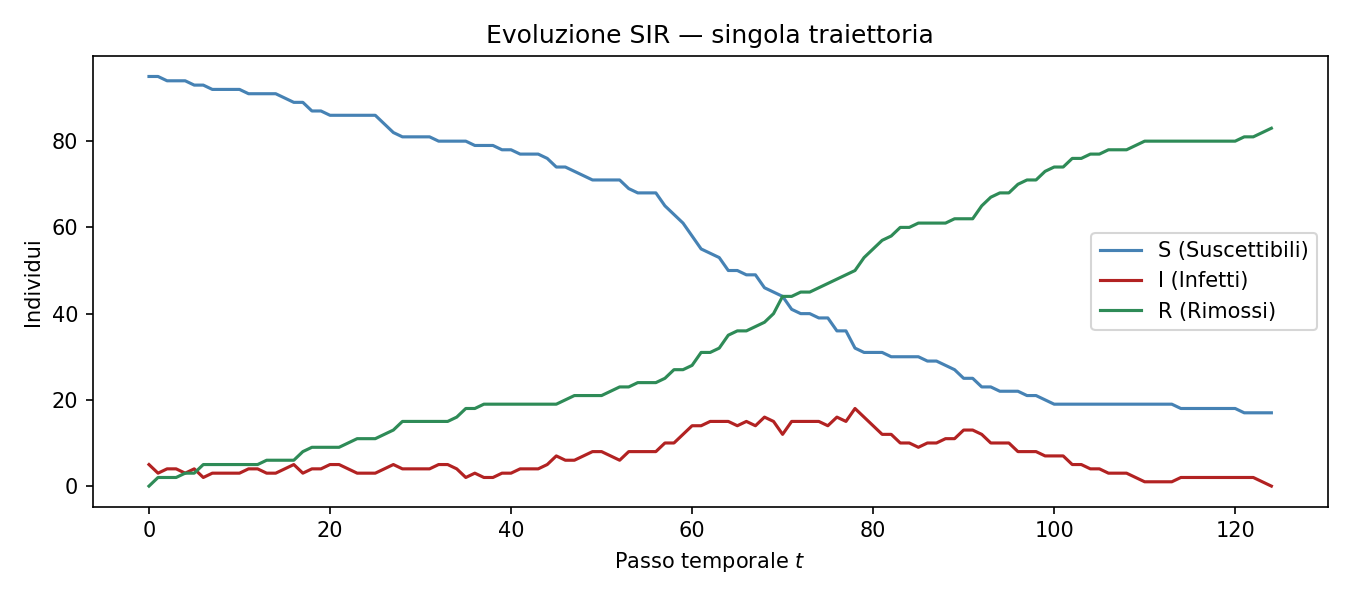
\includegraphics[width=0.7\textwidth]{../img/single_trajectory.png}
    \end{center}
    \begin{itemize}
        \item Curva blu ($S$): decresce irregolarmente.
        \item Curva rossa ($I$): sale al picco, poi scende a zero.
        \item Curva verde ($R$): cresce monotonamente fino a saturazione.
    \end{itemize}
    \textit{La stocasticità è visibile nell'irregolarità delle curve.}
\end{frame}

% SLIDE 15
\begin{frame}{Traiettoria media $\pm$ 1 dev. std}
    \begin{center}
        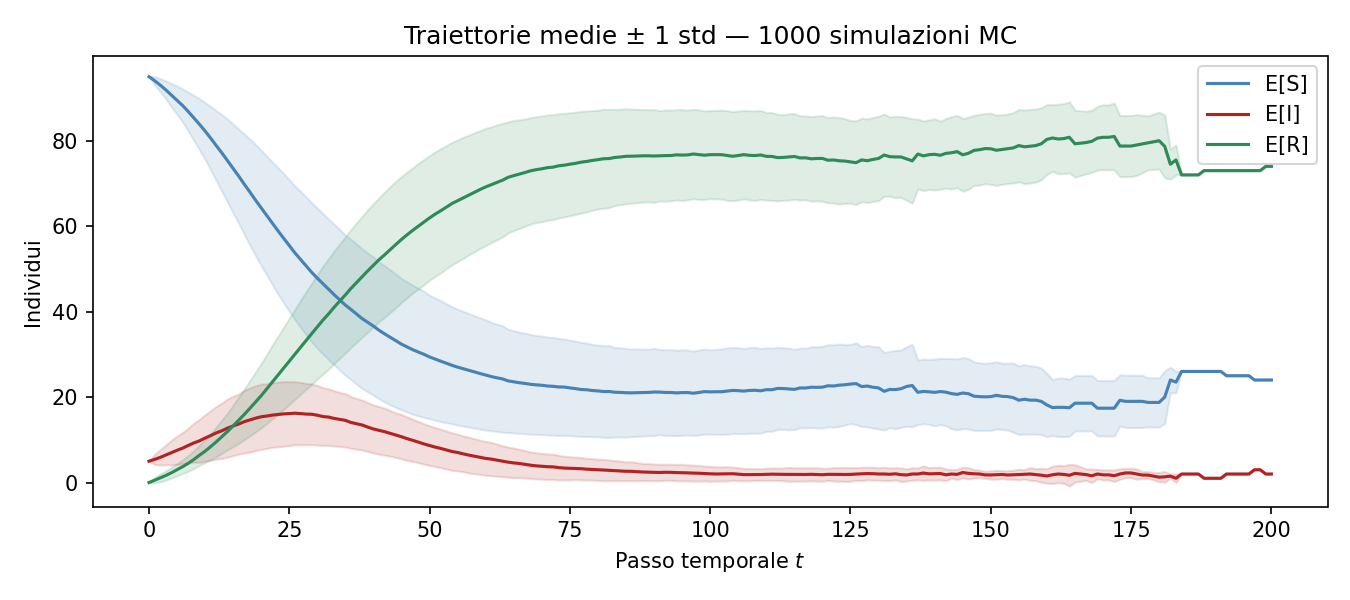
\includegraphics[width=0.7\textwidth]{../img/mean_trajectory.png}
    \end{center}
    \begin{itemize}
        \item Linee continue: medie su 1000 simulazioni.
        \item Aree trasparenti: $\pm 1$ deviazione standard.
        \item Variabilità massima nella fase di picco.
    \end{itemize}
\end{frame}

% SLIDE 16
\begin{frame}{Distribuzione del tempo di estinzione $\tau$}
    \begin{center}
        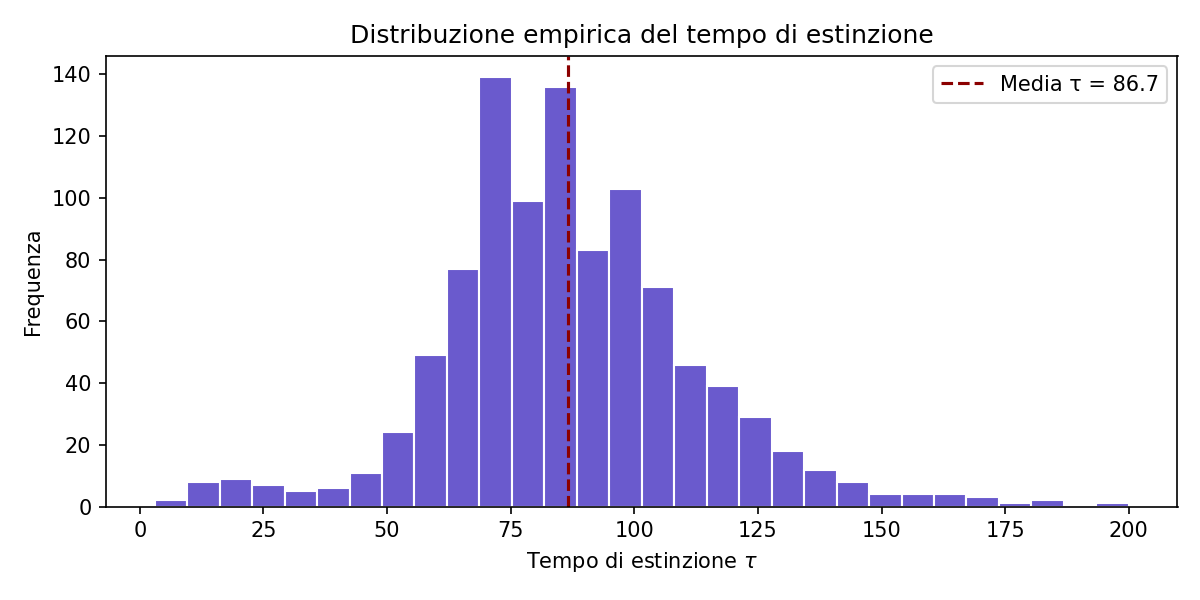
\includegraphics[width=0.7\textwidth]{../img/tau_histogram.png}
    \end{center}
    \begin{itemize}
        \item Forma campanulare con coda destra.
        \item Asimmetria positiva: alcune epidemie durano molto più della media.
        \item \textit{Distribuzione empirica stimata via Monte Carlo.}
    \end{itemize}
\end{frame}

% SLIDE 17
\begin{frame}{Interpretazione}
    \begin{enumerate}
        \item \textbf{Estinzione certa}: 100\% delle simulazioni $\rightarrow$ catena assorbente.
        \item \textbf{Variabilità}: scarto tipo del picco $= 8.7$ su media $29.4$.
        \item \textbf{Picco}: $\sim 29\%$ della popolazione infetta contemporaneamente.
        \item \textbf{$R_\infty$ medio}: $87\%$ della popolazione contratta l'infezione. (Coerente con $R_0 = 2$).
    \end{enumerate}
\end{frame}

% SLIDE 18
\begin{frame}{Teoria vs Simulazione}
    \begin{center}
    \begin{tabular}{ll}
        \toprule
        Previsione teorica & Verifica simulativa \\
        \midrule
        Assorbimento certo ($\Prob(\tau < \infty)=1$) & \checkmark 1000/1000 casi \\
        $\tau = \text{soluzione di } (I-Q)\mathbf{t} = \uno$ & \checkmark $\tau \text{ medio} \approx 68$ (stimato) \\
        $R_\infty$ è una variabile casuale & \checkmark Distribuzione empirica ottenuta \\
        \bottomrule
    \end{tabular}
    \end{center}
    
    \vspace{0.5cm}
    \textbf{Punto chiave}: La simulazione NON sostituisce la teoria. La simulazione \textbf{stima} quantità che la teoria definisce matematicamente. È la teoria che dà significato ai numeri.
\end{frame}

% SLIDE 19
\begin{frame}{Limiti del modello}
    \begin{center}
    \begin{tabular}{ll}
        \toprule
        Limite & Impatto \\
        \midrule
        Popolazione chiusa & Ignora dinamiche demografiche \\
        $\beta, \gamma$ costanti & Ignora stagionalità e interventi \\
        Mescolamento omogeneo & Ignora reti sociali reali \\
        Nessuna reinfezione & Non sempre realistico \\
        \bottomrule
    \end{tabular}
    \end{center}
    
    \vspace{0.5cm}
    \textbf{Ma}: questi limiti sono \textbf{voluti}. Il fine primario non è prevedere un'epidemia reale, ma fornire un \textit{sandbox} rigoroso per il formalismo delle Catene di Markov.
\end{frame}

% SLIDE 20
\begin{frame}{Sviluppi futuri}
    \begin{itemize}
        \item \textbf{Modello SIS o SIRS}: reintrodurre i guariti nei suscettibili per studiare l'endemicità (la catena non sarebbe più assorbente).
        \item \textbf{Parametri tempo-dipendenti}: $\beta(t)$ per simulare interventi non farmacologici (lockdown).
        \item \textbf{Matrice sparsa}: costruire la matrice $P$ esplicita per $N=100$ sfruttando la sparsità, per calcolare la soluzione esatta del sistema $(I-Q)\mathbf{t} = \uno$ invece che per via simulativa.
    \end{itemize}
\end{frame}

% SLIDE 21
\begin{frame}{Conclusioni}
    \begin{itemize}
        \item Il formalismo delle \textbf{Catene di Markov a tempo discreto} fornisce una cornice matematica solida per lo studio di processi stocastici discreti come il modello SIR su popolazioni finite.
        \item Sebbene le matrici transitorie per $N$ grande siano analiticamente intrattabili, le \textbf{proprietà teoriche} (ad es. l'assorbimento quasi-certo per $I=0$) rimangono i pilastri su cui si basano le simulazioni.
        \item I metodi \textbf{Monte Carlo} offrono un ponte concreto per campionare questo spazio degli stati e derivare stime empiriche robuste.
    \end{itemize}
    
    \vspace{0.8cm}
    \begin{center}
        \Large{\textbf{Grazie per l'attenzione!}}
    \end{center}
\end{frame}

\end{document}
